% This is "sig-alternate.tex" V2.1 April 2013
% This file should be compiled with V2.5 of "sig-alternate.cls" May 2012
%
% This example file demonstrates the use of the 'sig-alternate.cls'
% V2.5 LaTeX2e document class file. It is for those submitting
% articles to ACM Conference Proceedings WHO DO NOT WISH TO
% STRICTLY ADHERE TO THE SIGS (PUBS-BOARD-ENDORSED) STYLE.
% The 'sig-alternate.cls' file will produce a similar-looking,
% albeit, 'tighter' paper resulting in, invariably, fewer pages.
%
% ----------------------------------------------------------------------------------------------------------------
% This .tex file (and associated .cls V2.5) produces:
%       1) The Permission Statement
%       2) The Conference (location) Info information
%       3) The Copyright Line with ACM data
%       4) NO page numbers
%
% as against the acm_proc_article-sp.cls file which
% DOES NOT produce 1) thru' 3) above.
%
% Using 'sig-alternate.cls' you have control, however, from within
% the source .tex file, over both the CopyrightYear
% (defaulted to 200X) and the ACM Copyright Data
% (defaulted to X-XXXXX-XX-X/XX/XX).
% e.g.
% \CopyrightYear{2007} will cause 2007 to appear in the copyright line.
% \crdata{0-12345-67-8/90/12} will cause 0-12345-67-8/90/12 to appear in the copyright line.
%
% ---------------------------------------------------------------------------------------------------------------
% This .tex source is an example which *does* use
% the .bib file (from which the .bbl file % is produced).
% REMEMBER HOWEVER: After having produced the .bbl file,
% and prior to final submission, you *NEED* to 'insert'
% your .bbl file into your source .tex file so as to provide
% ONE 'self-contained' source file.
%
% ================= IF YOU HAVE QUESTIONS =======================
% Questions regarding the SIGS styles, SIGS policies and
% procedures, Conferences etc. should be sent to
% Adrienne Griscti (griscti@acm.org)
%
% Technical questions _only_ to
% Gerald Murray (murray@hq.acm.org)
% ===============================================================
%
% For tracking purposes - this is V2.0 - May 2012
\documentclass{sig-alternate-05-2015}

\usepackage{graphicx}

\begin{document}

% Copyright
%\setcopyright{acmcopyright}
%\setcopyright{acmlicensed}
%\setcopyright{rightsretained}
%\setcopyright{usgov}
%\setcopyright{usgovmixed}
%\setcopyright{cagov}
%\setcopyright{cagovmixed}


% DOI
%\doi{10.475/123_4}

% ISBN
%\isbn{123-4567-24-567/08/06}

%Conference
%\conferenceinfo{PLDI '13}{June 16--19, 2013, Seattle, WA, USA}

%s\acmPrice{\$15.00}

%
% --- Author Metadata here ---
%\conferenceinfo{WOODSTOCK}{'97 El Paso, Texas USA}
%\CopyrightYear{2007} % Allows default copyright year (20XX) to be over-ridden - IF NEED BE.
%\crdata{0-12345-67-8/90/01}  % Allows default copyright data (0-89791-88-6/97/05) to be over-ridden - IF NEED BE.
% --- End of Author Metadata ---

\title{Analysis of the efficiency and user satisfaction of a menu and swipe gestures in the context of a survey app}

%
% You need the command \numberofauthors to handle the 'placement
% and alignment' of the authors beneath the title.
%
% For aesthetic reasons, we recommend 'three authors at a time'
% i.e. three 'name/affiliation blocks' be placed beneath the title.
%
% NOTE: You are NOT restricted in how many 'rows' of
% "name/affiliations" may appear. We just ask that you restrict
% the number of 'columns' to three.
%
% Because of the available 'opening page real-estate'
% we ask you to refrain from putting more than six authors
% (two rows with three columns) beneath the article title.
% More than six makes the first-page appear very cluttered indeed.
%
% Use the \alignauthor commands to handle the names
% and affiliations for an 'aesthetic maximum' of six authors.
% Add names, affiliations, addresses for
% the seventh etc. author(s) as the argument for the
% \additionalauthors command.
% These 'additional authors' will be output/set for you
% without further effort on your part as the last section in
% the body of your article BEFORE References or any Appendices.

\numberofauthors{4} %  in this sample file, there are a *total*
% of EIGHT authors. SIX appear on the 'first-page' (for formatting
% reasons) and the remaining two appear in the \additionalauthors section.
%
\author{
% You can go ahead and credit any number of authors here,
% e.g. one 'row of three' or two rows (consisting of one row of three
% and a second row of one, two or three).
%
% The command \alignauthor (no curly braces needed) should
% precede each author name, affiliation/snail-mail address and
% e-mail address. Additionally, tag each line of
% affiliation/address with \affaddr, and tag the
% e-mail address with \email.
%
% 1st. author
\alignauthor 
Lukas Galke\\
       \email{mail@uni-kiel.de}
% 2nd. author
\alignauthor Steffen Goos\\
      \email{mail@uni-kiel.de}
% 3rd. author
\alignauthor
Felix Paur\\
       \email{mail@uni-kiel.de}
\and  % use '\and' if you need 'another row' of author names
% 4th. author
\alignauthor
Florian Mai\\
       \email{mail@uni-kiel.de}
}
% There's nothing stopping you putting the seventh, eighth, etc.
% author on the opening page (as the 'third row') but we ask,
% for aesthetic reasons that you place these 'additional authors'
% in the \additional authors block, viz.
%\additionalauthors{Additional authors: John Smith (The Th{\o}rv{\"a}ld Group,
%email: {\texttt{jsmith@affiliation.org}}) and Julius P.~Kumquat
%(The Kumquat Consortium, email: {\texttt{jpkumquat@consortium.net}}).}
%\date{30 July 1999}
% Just remember to make sure that the TOTAL number of authors
% is the number that will appear on the first page PLUS the
% number that will appear in the \additionalauthors section.

\maketitle
\begin{abstract}
For several years, the swipe gesture has been a very-well established way to navigate among adjacent pages on websites as well as in native
apps on a mobile device. The users appreciate its ease and its comfort of use. However, it can only be applied in scenarios where
the content is provided in a sequential way, e.g. in a picture gallery, in an e-book reader, or when filling in a form. In this paper, we
examine the swipe gesture's suitability for navigating through a set of question in a survey. Although typically the user progresses 
through the questions sequentially, it is a common case that they want to revise their answers later due to a change of mind or a missunderstanding
of the question, for example. We conjecture that navigating back using swipe gestures is unsatisfactory and time-costly as the distance in pages
increases. In order to research this question, we conduct a study in which we compare the use of swipe gestures to the use of the also
well-established hamburger menu. We design tasks that capture the use cases described above. We alter the distance in pages
that has to be covered in order to complete the task. For each task, we measure the efficiency. Furthermore, we assess the user satisfaction through a questionnaire. We expect
both measures to be independent of the distance when the menu is used. When the swipe gesture is used, however, we expect both measures to decrease
as the distance increases. We suspect that the swipe gestures do better than the menu when the distance is small, but we also think that this
this relation flips at a number of pages that is realistic for surveys. Hence, the results of our study are of practical importance.
\end{abstract}


%
% The code below should be generated by the tool at
% http://dl.acm.org/ccs.cfm
% Please copy and paste the code instead of the example below. 
%
\begin{CCSXML}
<ccs2012>
 <concept>
  <concept_id>10010520.10010553.10010562</concept_id>
  <concept_desc>Computer systems organization~Embedded systems</concept_desc>
  <concept_significance>500</concept_significance>
 </concept>
 <concept>
  <concept_id>10010520.10010575.10010755</concept_id>
  <concept_desc>Computer systems organization~Redundancy</concept_desc>
  <concept_significance>300</concept_significance>
 </concept>
 <concept>
  <concept_id>10010520.10010553.10010554</concept_id>
  <concept_desc>Computer systems organization~Robotics</concept_desc>
  <concept_significance>100</concept_significance>
 </concept>
 <concept>
  <concept_id>10003033.10003083.10003095</concept_id>
  <concept_desc>Networks~Network reliability</concept_desc>
  <concept_significance>100</concept_significance>
 </concept>
</ccs2012>  
\end{CCSXML}

\ccsdesc[500]{Computer systems organization~Embedded systems}
\ccsdesc[300]{Computer systems organization~Redundancy}
\ccsdesc{Computer systems organization~Robotics}
\ccsdesc[100]{Networks~Network reliability}


%
% End generated code
%

%
%  Use this command to print the description
%
\printccsdesc

% We no longer use \terms command
%\terms{Theory}

\keywords{ACM proceedings; \LaTeX; text tagging}

\section{Introduction}
For several years, the swipe gesture has been a very-well established way to navigate among adjacent pages on websites as well as in native
apps on a mobile device. The users appreciate its ease and its comfort of use. However, it can only be applied in scenarios where
the content is provided in a sequential way, e.g. in a picture gallery, in an e-book reader, or when filling in a form. In this paper, we
examine the swipe gesture's suitability for navigating through a set of question in a survey. Although typically the user progresses 
through the questions sequentially, it is a common case that they want to revise their answers later due to a change of mind or a missunderstanding
of the question, for example. We conjecture that navigating back using swipe gestures is unsatisfactory and time-costly as the distance in pages
increases. In order to research this question, we conduct a study in which we compare the use of swipe gestures to the use of the also
well-established hamburger menu. We suspect that the swipe gestures do better in terms of efficiency, (effectiveness), and
user satisfaction than the hamburger menu when the distance is small. When the distance is large, however,
we believe that this relation flips. More formally, let $d$ be the distance in pages to be covered when navigating in a sequence of pages.
We formulate the following hypotheses:
\begin{enumerate}
  \item Null hypothesis $H_0^{(e)}$ for efficiency: There is no difference in efficiency between swipe gestures and hamburger menu when navigating over a distance of $d$ pages.
  \item Alternative hypothesis $H_1^{(e)}$ for efficiency: There is a difference in efficiency between swipe gestures and hamburger menu when navigating over a distance of $d$ pages.
  \item Null hypothesis $H_0^{(s)}$ for user satisfaction: There is no difference in user satisfaction between swipe gestures and hamburger menu when navigating over a distance of $d$ pages.
  \item Alternative hypothesis $H_1^{(s)}$ for user satisfaction: There is a difference in user satisfaction between swipe gestures and hamburger menu when navigating over a distance of $d$ pages.
\end{enumerate}
In fact, we check these hypotheses for different values of $d$. We talk to experts from the educational science domain to identify values for $d$ that are realistic for the scenarios described above.
\section{Related Work}

\section{Study Design}
\subsection{Conceptual Design}
\subsubsection{Hypothesis}

Between-Group Design or Within-Group-Design?
\subsubsection{Participants}
\subsubsection{Tasks}
In order to simulate the scenarios of jumping from one question to another, we developed a series of puzzle-like tasks. The goal is to find a
keyword solution composed of five letters. An instruction displayed on the bottom of the screen guides the participant to the next letter. It always asks the
participant to navigate to some question and pick a certain character on the screen as the next letter. When the participant has entered a letter, the next
instruction is displayed. The distance to cover from one question to another is always in the same small range for each quiz. However, the distances differ for
different quizzes. As an example, consider the example in Figure \ref{fig:puzzle} which has distances in range two to three. The arrows indicate the question to jump to in
the next step and the number attached to the labels indicates which character in the question is the next letter. Hence, in this example, the solution is 'nupvr'.
\begin{figure}
\caption{An example of a puzzle}
\resizebox{\columnwidth}{!}{
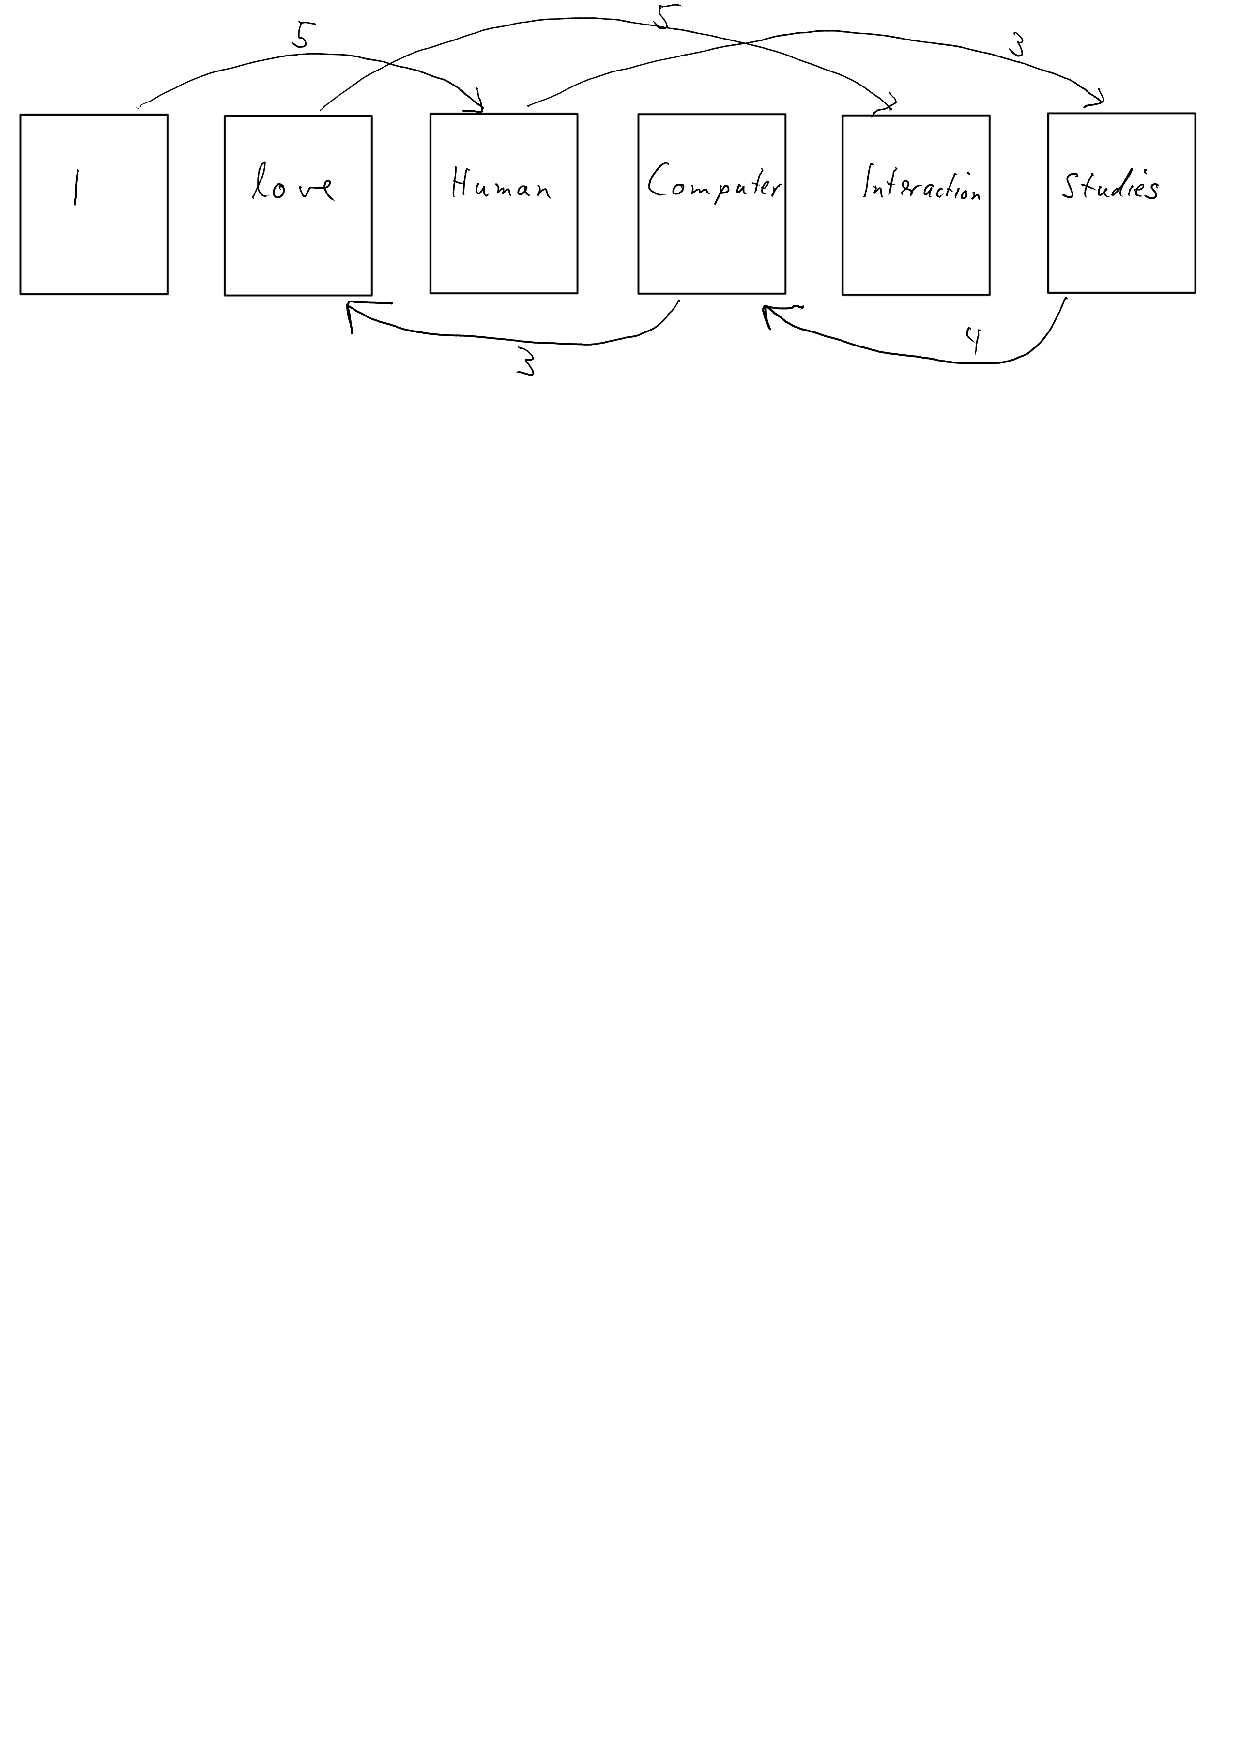
\includegraphics[clip, trim=0cm 23cm 0cm 0cm]{schnitzeljagd.pdf}
\label{fig:puzzle}
}
\end{figure}
\subsubsection{Measures}
As stated above, we aim to measure the effectiveness, efficiency, and satisfaction of the two navigation methods. 
\paragraph{Effectiveness} Effectiveness is estimated as the portion of
correctly picked letters. 
\paragraph{Efficiency} For the efficiency, we only measure the time required to get to the page on which the next letter can be found. We start measuring at the point
when the previous letter has been entered.
\paragraph{Satisfaction}
In order to assess the user satisfaction depending on the distance, the user is asked to fill in a short questionnaire after each puzzle. 
The questionnaire consists of the following questions:
\begin{enumerate}
  \item How did you enjoy the puzzle?
  \item How tired did you get during solving the puzzle?
  \item \ldots
\end{enumerate}
\subsection{Realization of the Experiment}
We developed a simple Android application:
\subsubsection{GUI}
put a qt mock-up here
\subsubsection{How we measured efficiency (and effectiveness)}
maybe we don't need this
\section{Experiments and Results}
\section{Discussion}

\section{Conclusions}
Conclusions
%\end{document}  % This is where a 'short' article might terminate

%ACKNOWLEDGMENTS are optional
\section{Acknowledgments}
This section is optional; it is a location for you
to acknowledge grants, funding, editing assistance and
what have you.  In the present case, for example, the
authors would like to thank Gerald Murray of ACM for
his help in codifying this \textit{Author's Guide}
and the \textbf{.cls} and \textbf{.tex} files that it describes.

%
% The following two commands are all you need in the
% initial runs of your .tex file to
% produce the bibliography for the citations in your paper.
\bibliographystyle{abbrv}
\bibliography{hci}  % sigproc.bib is the name of the Bibliography in this case
% You must have a proper ".bib" file
%  and remember to run:
% latex bibtex latex latex
% to resolve all references
%
% ACM needs 'a single self-contained file'!
%
%APPENDICES are optional
%\balancecolumns
\appendix
%Appendix A
\section{Some Appendices}
\end{document}
